\documentclass{article}
\usepackage{pgfplots}
\pgfplotsset{compat=newest}


%% the following commands are sometimes needed
\usetikzlibrary{plotmarks}
\usepackage{grffile}
\usepackage{booktabs}
%\usepackage{tikzpicture}
\usepackage{tikzscale}
\usepackage{fancyhdr}
\usepackage[cmex10]{amsmath}
\usepackage{mdwmath}
\usepackage{mdwtab}
\hyphenation{op-tical net-works semi-conduc-tor}
\usepackage{graphicx}
\usepackage{color}
\usepackage{placeins}
\usepackage{float}
\usepackage{hyperref}
\usepackage{tabularx,colortbl}
\usepackage{pgfplots}
\usepackage{subfig}
\usepackage{tikz}
\usepackage{tikz-3dplot}
\usepackage{booktabs}
\usepackage{standalone}
\usepackage{filecontents}


\begin{document}
	\title{Vertical Electric Dipole Above a Dielectric Half-space}
	\maketitle
	\begin{figure}[h]
		% \begin{centering}
		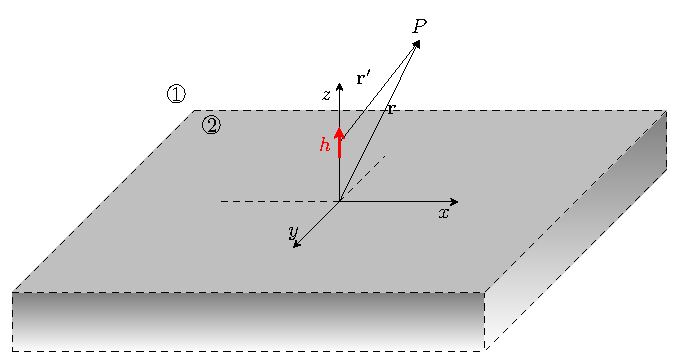
\includegraphics[scale=1]{VED_above_half_space.tex}
		% \end{centering}
		\caption{A vertically oriented Hertzian dipole above a dielectric half-space}
		\label{fig:VED}
	\end{figure}

An infinitesimally small electric dipole is vertically oriented in free space (medium 1) at $z = h$ and lies above a dielectric half space (medium 2). The media interface is at $ z = 0$. An observation point $P$ is chosen as illustrated in Fig. \ref{fig:VED}. The current on the dipole is expressed as,
\begin{equation}
	\mathbf{J} = Il  \delta(x) \delta(y) \delta(z-h) \bf{\hat{z}}
	\label{eq:J}
\end{equation}
where the product of current $I$ and length $l$ gives the dipole moment.

Before formulating the problem, we express the propagation constant in each medium,
\begin{subequations}
\begin{equation}
	\begin{split}
	k_1 & = \omega \mu_1 \varepsilon_1 \\
		& = \omega \mu_0 \varepsilon_0,
	\end{split}
	\label{eq:k_1}
\end{equation}
\begin{equation}
	\begin{split}
	k_2 & = \omega \mu_2 \varepsilon_2 \\
 		& = \omega \mu_0 \varepsilon_0 \left( \varepsilon' - j\varepsilon '' \right).
	\end{split}
	\label{eq:k_2}
\end{equation}
\end{subequations}
Here we consider the dielectric to be non-magnetic and lossy which is manifested by a complex dielectric constant. In order to find the solution of the radiation problem at hand, we first look at the Maxwell's equations,
\begin{subequations}
	\begin{equation}
		\nabla\cdot{\bf D} = \rho,
		\label{eq:gauss}
	\end{equation}
		\begin{equation}
		 \nabla\cdot{\bf H} = 0,
		\label{eq:gauss_h}
	\end{equation}
		\begin{equation}
		\nabla\times{\bf E} = - \mu{{\partial{ \bf H}}\over{\partial t}},
		\label{eq:faraday}
	\end{equation}
		\begin{equation}
		\nabla\times{\bf H} = {\bf J} + \varepsilon{{\partial{ \bf E}}\over{\partial t}}.
		\label{eq:amperes}
	\end{equation}
\end{subequations}

It is convenient to introduce magnetic vector potential, $\mathbf A$ at this point and set up the corresponding Helmholtz equation,
\begin{subequations}
	\begin{equation}
			\begin{split}
		\left( \nabla^2 + k^2 \right) \mathbf{A}  & = -\mu \mathbf{J} \\
			& = -\mu Il \delta(x) \delta(y) \delta(z-h) \bf{\hat{z}},  z > 0
		\end{split}
	\end{equation}
	\begin{equation}
		\left(\nabla^2 + k^2 \right) \mathbf{A}  = 0, z < 0.
	\end{equation}
	\label{eq:helmholtz}
\end{subequations}
The electric and magnetic fields can be expressed in term of the potential function, $\mathbf A$ as:
\begin{subequations}
	\begin{equation}
		\mathbf{E} = -\frac{j\omega}{k^2}\left( k^2 + \nabla \nabla \cdot \right) \mathbf{A},
		\label{eq:EinA}
	\end{equation}
		\begin{equation}
		 \mathbf{H} = \frac{1}{\mu}\nabla\times{\bf A}.
		\label{eq:HinA}
	\end{equation}
\end{subequations}

In order to solve (\ref{eq:helmholtz}), continuity of tangential components of electric and magnetic fields is considered. The electric and magnetic fields can be resolved into Cartesian components as:
       \begin{align*}
        & E_x = -\frac{j\omega}{k^2}\frac{\partial^2 A_z}{\partial z^2} && H_x = \frac{1}{\mu}\frac{\partial A_z}{\partial y} \\
        & E_y = -\frac{j\omega}{k^2}\frac{\partial^2 A_z}{\partial y \partial z} && H_y = -\frac{1}{\mu}\frac{\partial A_z}{\partial x} \\
        & E_z = -\frac{j\omega}{k^2}\left( k^2 +\frac{\partial^2 A_z}{\partial z^2} \right) && H_z = 0.
        \end{align*}


\end{document}  

